\section{Approach}

\textbf{Cost Model.} In general, we consider any program as a function of some input, some of which may be marked as private or secret. Any run of the function returns an observable value which represents the side channel measurements of that execution of function. 

Given a type of side channel, we can develop a cost model to approximate the output of that channel along a control flow path. For a given instruction, a cost model returns an expression for the observable of the considered channel. For example, a cost model for timing side channels might return the number of bytecode instructions, which can be used a proxy for execution time. These cost models provide static approximations of the observables that can be determined without running the program under test. Note that two executions of the same program with the same input might produce different observables --- for example, the execution time may be slightly different --- but the cost associated with their path through the control flow graph under the given cost model will remain the same.



\textbf{Path Cost Analysis.} The control flow graph of a program is a representation of all paths that might be traversed through a program during its execution. It is defined as a directed graph $G = (V, E)$ where the set of vertices $V$ are basic blocks and the set of edges $E$ represent jumps in the control flow. Path cost analysis is a technique we introduce to generate a symbolic expression for each node and back edge of the control flow graph which gives an over-approximation on the set of possible observable values at that node or for that cycle. Pairs of these symbolic cost expressions will be compared in order to detect paths in the control flow graphs that are imbalanced with respect to the given cost model. 


 %Our goal is to efficiently search the control flow graph for paths that are imbalanced with respect to our given cost model. Such an imbalance in the control flow graph marks a potential side channel in the method. To detect imbalanced paths, we introduce a method to annotate each node of the control flow graph with an expression that gives all potential cost values at the node, given a certain starting point. 
We do not analyze the entire control flow graph at once. Instead we perform an iterative analysis, first annotating smaller subgraphs and then combining the results to detect imbalance across these subgraphs. Our subgraphs are defined by the nesting structure of cycles in the control flow graph. If the control flow graph contains cycles, we annotate them first. Annotation of any cycle begins by recursively annotating its nested cycles. The base cases are cycles that contain no other cycles. To annotate a such a cycle, first remove the back edge, making an acyclic subgraph. It is now annotated as any other acyclic subgraph of the program. 

\textit{Annotation of Acyclic Graph:} To annotate an acyclic subgraph, we consider its nodes in topological order. The cost expression, $c_n$ of a node, $n$, is determined from the cost expressions of $n$'s immediate predecessors. Since $n$ represents a basic block of the method, let $|n|$ be the cost of this basic block under the given cost model (i.e. the number of bytecode instructions in $n$).  If $n$ has no predecessors, then $c_n$ is simply $|n|$.  If $n$ has one immediate predecessor, then its cost expression is the addition of $|n|$ and the cost expression of $n$'s immediate predecessor. If $n$ has two or more immediate predecessors, then two or more branches are merged at $n$. We will analyze the merging of each pair of branches individually. To do this, we will insert an additional node into the control flow graph for each additional merge in order of the most recently branched. These additional nodes will each have two incoming edges as will the original $n$. The cost expression for a node with two immediate predecessors is the addition of $|n|$ to $b \cdot c_{n-1} + (1 - b) \cdot c_{n-2}$, where nodes $n-1$ and $n-2$ are the two immediate predecessors of $n$ and $b$ is a fresh boolean variable. In this way, each branch condition is associated with a boolean variable, which represents whether the left of right branch was taken. See Fig~\ref{fig:merge} for the annotation of an acyclic subgraph with three paths merging at one node. The green node was added to the graph in order to merge the more recent left branch before the right. 

\begin{figure}
  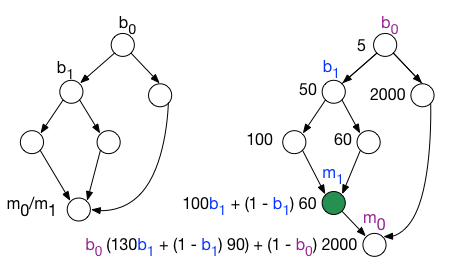
\includegraphics[scale=.5]{merge_paths.png}
  \caption{Left: original control flow graph. Right: annotated control flow graph.}
  \label{fig:merge}
\end{figure}

\vspace*{-0.1in} 


The only operation needed to generate the cost expression for a node in an acyclic graph is the addition of an integer to a cost expression. All possible cost expressions in an acyclic graph are given by:

$$Expr \rightarrow \begin{cases} Int  \\ b \cdot Expr_{0} + (1 - b) \cdot Expr_{1} \end{cases}$$

where b is a boolean variable, and $Expr_0$ and $Expr_1$ are the two possible cost expressions based on which branch to the most recent merge was taken. Addition by an integer is defined in each case as 

 $$Expr + Int \rightarrow \begin{cases} Int + Int \\ b \cdot (Expr_0 + Int) + (1 - b) \cdot (Expr_1 + Int) \end{cases}$$
  

%Since every node can only have up to two incoming edges and since the nodes of any non-cyclic graph can be annotated so that all predecessors of a node are annotated before that node, the above details a complete method for annotating the nodes of a non-cyclic subgraph.

\textit{Annotation of a Cyclic Subgraph.} The removed back edge is reintroduced and we derive its cost expression. We introduce a fresh integer variable $k$ denoting the number of times the cycle is taken. The cost expression of the cycle is now given by the product of the positive integer variable $k$ and the expression associated with the last node of the cycle. Multiplication by a integer variable is defined as 

 $$k \cdot Expr \rightarrow \begin{cases}  k \cdot Int \\ h \cdot Expr + (k - h) \cdot Expr \\\end{cases}$$
 
$h$ is a fresh variable which denotes the number of times out of the $k$ iterations of the cycle that a certain branch is taken. See Fig~\ref{fig:imb} for an example of how to annotate the back edge of a cycle.

\begin{figure}
  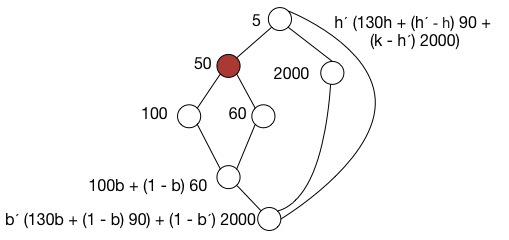
\includegraphics[scale=.5]{imbalance.png}
  \caption{Annotated control flow graph with a cycle. Red node is a branch on a secret variable.}
  \label{fig:imb}
\end{figure}

Finding the cost expressions for all nodes and back edges of a control flow graph can now be described as follows -- first recursively find the costs of all nested cycles, then treat each nested cycle as a single node for which $|n|$ is given by the cost of the cycle. This extends the set of possible cost expressions to include 

$$Expr \rightarrow \begin{cases} k \cdot Int  \\ h \cdot Expr_{0} + (k - h) \cdot Expr_{1} \end{cases}$$

and the rules for addition by an integer or multiplication by another loop variable are extended appropriately. 
 
\textbf{Imbalance Detection.} Given the annotated control flow graph, we compare select pairs of cost expressions to detect the presence of imbalanced control flow paths. These cost expressions are compared using a satisfiability solver such as z3 \cite{z3} or cvc4 \cite{cvc4} to determine whether there are satisfying solutions of their variables for which the distance between the two costs is higher than some user-provided threshold. There are three types of pairs of cost expressions to compare. 

1)\textit{ Output nodes.} Output nodes are any nodes in the control flow graph at which the observable may be measured when running the program. For example, any node where a packet is sent over the network is an instance of where an observable such as time or packet size could be collected. Not all output nodes need be compared with each other. To determine which output nodes to compare, we search the control flow graph to determine the set of \textit{output predecessors} for each output node. A node $p$ is an output predecessor of node $n$ if $p$ is either itself an output node or a node with no incoming edges and there is some path to $n$ including $p$ such that between some occurrence of $p$ and $n$, there is no other output node. Note that in the presence of loops, $n$ can be a predecessor of itself. Two non-identical output nodes are compared only in the case that intersection of their predecessor nodes is nonempty. An output node is compared with itself if there are two distinct paths to the output node with identical predecessors.  

2) \textit{ Secret Dependent Branch Conditions}  A branch condition is said to be dependent on a secret value if the value of any of its variables can be affected by the secret. For any branch condition in the control flow graph that depends on the secret value and does not form a back edge, we compare the cost expressions of the immediate predecessors of the node that merges the paths resultant from this branch. For any cycle in the control flow graph containing a conditional statement that depends on the secret value, we compare two copies of the cost expression of its back edge, each with its own set of fresh variables. 

% Likewise, for each back edge of the control flow graph, we consider the symbolic cost of the associated cycle and query the satisfiability solver to determine whether there are two distinct paths through the cycle such that the difference between the costs is greater than the threshold. 


%This result informs us as to whether there are two distinct paths in the control flow graph to the considered merge that are sufficiently imbalanced under the given cost model according to some threshold.

%This threshold can depend on the cost model and the expected noise of the system. For example, if the side channel is deterministic such the size of an output file, then the threshold might simply be zero. However, in the case where there is some system noise associated with the side channel, such as execution time, a higher threshold might be appropriate. 

%The number of nodes compared in the control flow graph is constant in the number of conditionals in the program. There is one additional set of nodes to be compared, which we refer to as output nodes. Output nodes are any nodes in the control flow graph at which the observable may be measured when running the program. For example, any node where a packet is sent over the network is an instance of where an observable such as time or packet size could be collected. Not all output nodes need be compared with each other. To determine which output nodes to compare, we search the control flow graph to determine the set of predecessors for each output node. A node $p$ is an predecessor of node $n$ if $p$ is either itself an output node or a node with no incoming edges and there is some path to $n$ including $p$ such that between some occurence of $p$ and $n$, there is no other output node. Note that in the presence of loops, $n$ can be a predecessor of itself. Two non-identical output nodes are compared only in the case that intersection of their predeccesor nodes is nonempty. An output node is compared with itself if there are two distinct paths to the output node with identical predecessors.  

%Regardless of what kind of nodes the query is on, the result is not only a boolean response as to the presence of imbalanced paths through the control flow graph but also a satisfying solution as to which branch conditions differ produce a pair of imbalanced paths. However, there might be many imbalanced paths that do not leak any information about the secret variables. This is because none of the differing branch conditions have any relation to the secret variables. In order to make our analysis more precise, we combine it with taint analysis to mark each branch condition in the control flow graph as dependent on a secret value or independent. A conditional is said to be dependent on a secret value if the value of any of its variables can be effected by the secret.

In all cases, the query to the satisfiability solver is constrained as follows. Both paths must agree on any variable whose associated branch condition does not depend on the secret value. The pair of witness paths returned by the satisfiability solver will be distinct paths in the control flow graph that differ on at least one branch condition that is dependent on the secret. Since the two paths are differentiable with respect to our cost model, this is exactly what it means for a side channel to be present. 

Consider the case in Fig~\ref{fig:imb} for a threshold of 100. The only branch statement is  that depends on the secret is $b_1$, the red node. To see if this branch statement alone induces a side channel, we compare the costs of the immediate predecessors of $m_1$, 100 and 60, to see that this side channel is not strong enough to be detected for the threshold. Since the branch at the first node of the graph, $b_0$ is not dependent on the secret we do not have to compare the two predecessors of its merge $m_0$. Finally, we consider the cost of the back edge. In this case, we set the maximum number of loop iterations to three and impose the constraint, $k \leq 3$. We compare two versions of the symbolic cost of the back edge, each with its own set of variables. Since neither the value of first branch nor the loop condition depends on the secret, the values of $h_0$ and $k$ must match. Only the value of $h_1$ may differ. In this case, we discover that $k = 3, h_0 = 3,h_1 = 3$ and $k = 3, h_0 = 3, h_1 = 0$ give two paths through the control flow graph, differing only on the branch condition at the node marked $b_1$, for which the difference in cost is greater than the given threshold. 